\section{Self-Play SWE-RL}
\label{section:approach}

\subsection{Overview}
The core idea of \techfull (\tech) is to allow LLM agents to self-improve through an iterative cycle of solving self-generated bugs and creating more complex challenges.
As shown in \cref{fig:overview}, the same LLM policy is divided into two roles: a bug-injection agent and a bug-solving agent. Both roles have access to the same containerized environment and set of tools, such as Bash and an editor, but are presented with different task specifications and requirements,
where the implementation of the tool-using scaffold
follows \cwm~\cite{faircodegenteam2025cwmopenweightsllmresearch}.
In detail, the bug-injection agent receives a sandboxed environment of a raw codebase. Its task is to introduce a bug by producing an artifact containing the necessary files. The artifact's consistency---ensuring the bug is present and reproducible---is then validated through execution.
A bug artifact that passes the consistency checking is considered valid and is presented to the solver agent, where the final solution patches are validated against the tests defined by the bug, with failure attempts treated as ``higher-order'' bugs for the agent to make another attempt on a different context.
Eventually, the bug injection reward signal combines the consistency validation and solver results to incentivize better proposals, while the bug solving reward signal leverages the testing results.
The same underlying policy LLM is jointly updated on both signals.

\subsection{Input Assumptions}
A key design principle of \tech is to minimize the required prior knowledge about the codebase, making the approach broadly applicable to diverse software projects. We only assume access to a corpus of Docker~\cite{docker} images containing source code repositories with dependencies installed.
Notably, we do not assume access to test parsers, existing tests, commands to execute the test suite, or any prior knowledge about the programming language or test framework. The bug-injection agent is responsible for discovering how to run tests, creating test parsers, and understanding the test suite structure entirely through environmental interaction. This minimal assumption set ensures that \tech can be applied to arbitrary codebases with minimal setup overhead.


\subsection{Agentic Bug Injection}
\label{sec:bug_injection}

\paragraph{Bug artifact.}
We specify a software bug for both training and evaluation purposes as an artifact of files that can validate the existence of a bug and a fix, parse the test results, define the bug changes, and hide the bug by weakening existing tests. Concretely, it involves the following files:
\begin{itemize}
    \item \texttt{\bfseries test\_script.sh}: a bash script that runs the test suite to detect bugs and validate fixes.

    \item \texttt{\bfseries test\_files.txt}: a list of oracle test files that are always reset to their original version before running the test suite. After applying a model-generated patch, we run the test suite to verify correctness. Resetting the test files ensures evaluation integrity: even if an agent modifies or ``games'' the test files rather than properly fixing the bug, the original tests are restored for evaluation.

    \item \texttt{\bfseries test\_parser.py}: a Python script that parses test output and produces a detailed JSON mapping of each test ID to its result (\texttt{passed} / \texttt{failed}).
    The parser can be implemented in any programming language, irrelevant to the codebase's language; we use Python for its simplicity.

    \item \texttt{\bfseries bug\_inject.diff}: a git diff patch that introduces bugs into the existing codebase.

    \item \texttt{\bfseries test\_weaken.diff}:
    a git diff patch that removes or weakens tests to hide the bug from the test suite. This simulates realistic bugs that escape detection by existing tests and creates a test gap so that reversing it defines the expected behavior the fix must satisfy, serving as a specification for the solver. \Cref{fig:weakening} shows an example.

\end{itemize}

\begin{figure*}[htb!]
    \centering
    \begin{subfigure}{0.49\linewidth}
        \centering
        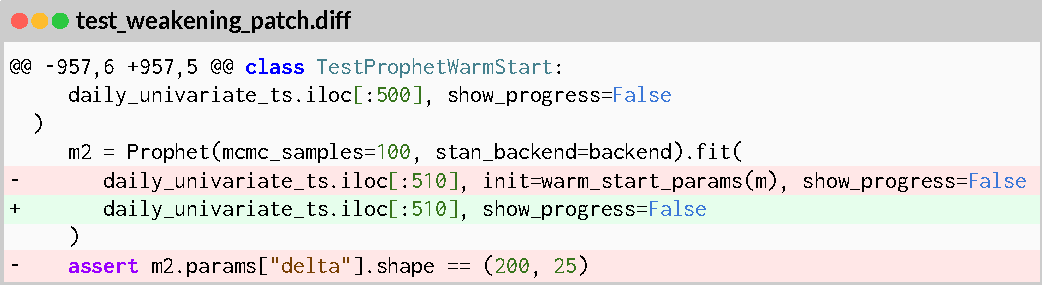
\includegraphics[width=\linewidth]{plots/ssr-test-weakening.pdf}
    \end{subfigure}%
    \hfill%
    \begin{subfigure}{0.49\linewidth}
        \centering
        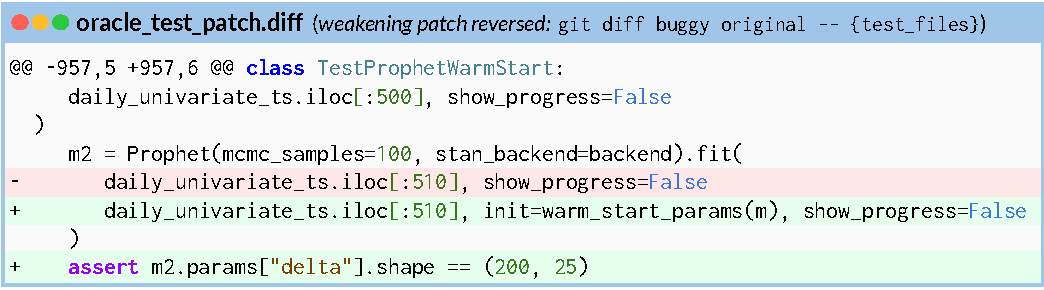
\includegraphics[width=\linewidth]{plots/ssr-test-weakening-reverse.pdf}
    \end{subfigure}
    \caption{Example test weakening patch and its reversal as the oracle test specification for the solver.}
    \label{fig:weakening}
\end{figure*}

\paragraph{Complex bug generation.}
In \tech, bug generation is an agentic task where the agent interacts with the execution environment with tools to produce a bug artifact, further validated for consistency and provided to the solver agent. Based on the reward signal obtained from consistency checking and the feedback from the solver agent, the bug-injection agent learns to create higher-quality bugs that are more consistent and tailored for the solver through RL.

\begin{figure*}[htb!]
    \centering
    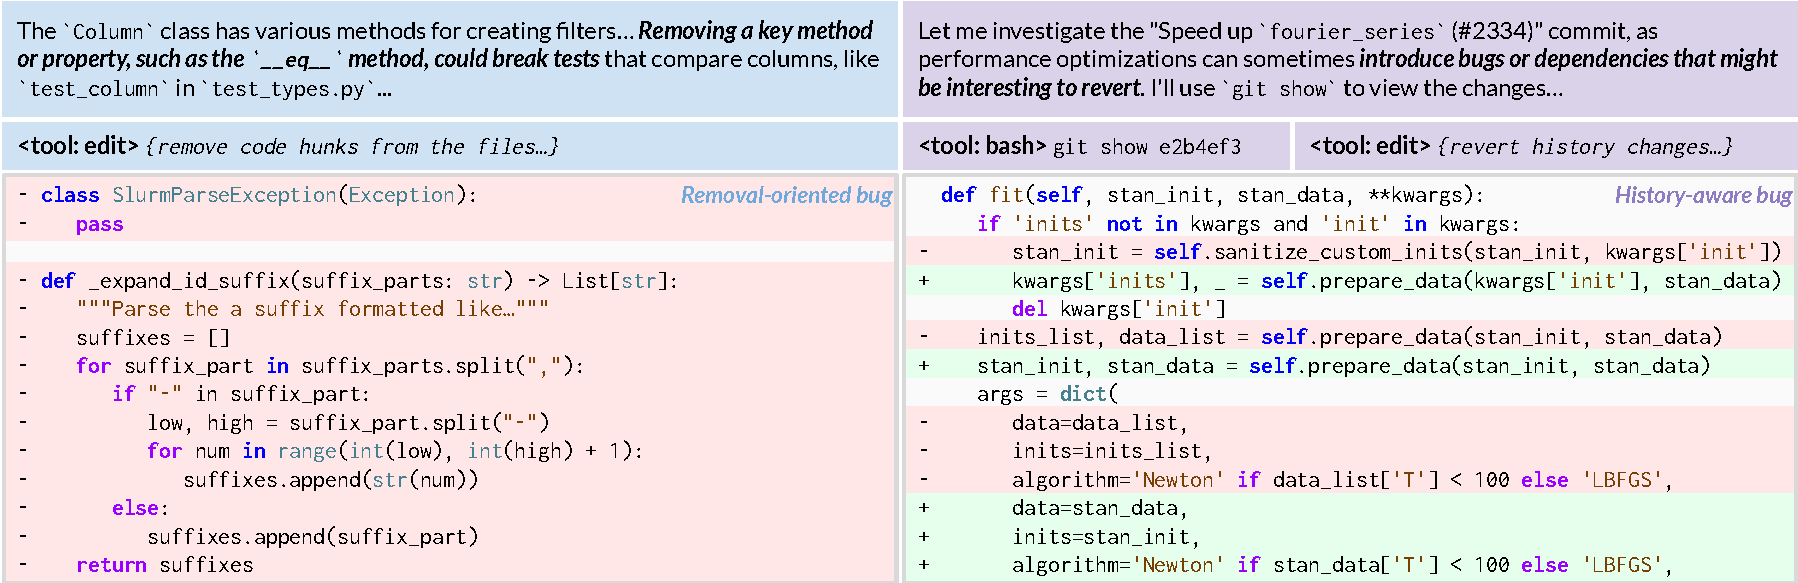
\includegraphics[width=\linewidth]{plots/ssr-bug-types.pdf}
    \caption{Bug-injection patches generated by code hunk removal (left) and historical change reversion (right).}
    \label{fig:bug-injection-methods}
\end{figure*}

One crucial property for a good bug-injection agent is its ability to generate diverse bugs that capture the complexity of real-world software development, thereby training the solver agent across a comprehensive spectrum of software debugging and engineering scenarios.
To achieve this, we adopt two simple strategies: instructing the agent to (1) \textbf{remove code files or hunks} from the codebase or (2) selectively \textbf{revert historical code changes} leveraging insights from git logs.
Fixing these bugs requires adding or modifying code, which are among the most frequent change types in real-world software evolution.
For both approaches, we require the agent to perform compatibility fixes to ensure the project remains runnable, so that any resulting bug reflects a true semantic error rather than a trivial syntax issue.
With these bug injection methods, the solver agent is forced to understand how the repository is built by recovering the correct original code from a broken codebase.
\Cref{fig:bug-injection-methods} shows the example bug-injection patches and the key reasoning and action traces for the two methods.

Additionally, we introduce some control parameters, such as the minimum number of changed files, passing tests, and failing tests after injection to ensure the quality and complexity of the bug.
See \cref{sec:apd:prompt_bug_injection} for the detailed prompts.


\paragraph{Consistency validation.}
Each first-order bug artifact is validated against a set of execution rules to ensure it is meaningful.
\Cref{fig:consistency-val}
shows some key steps. Below, we describe the complete checks:
\begin{figure*}[ht!]
    \centering
    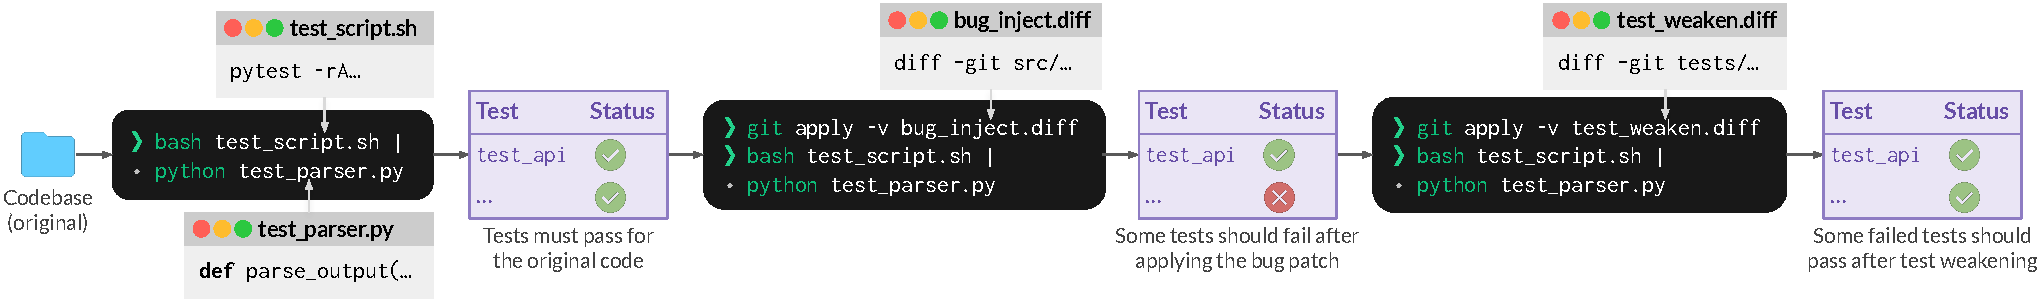
\includegraphics[width=\linewidth]{plots/ssr-consistency-val.pdf}
    \caption{Key consistency checks applied to validate bug artifacts, the full set described in the text.}
    \label{fig:consistency-val}
\end{figure*}
\begin{itemize}

    \item \textbf{Test files existence and coverage:} all the test files must exist in the original repository and must be a superset of the files touched by the test weakening patch.

    \item \textbf{Test parser validity:} the test parser \texttt{test\_parser.py}, used throughout subsequent validation steps, must reliably convert raw test output into a detailed JSON mapping from test names to their statuses (\texttt{passed} or \texttt{failed}).

    \item \textbf{Test script validity:} when executed on the original codebase, the test script \texttt{test\_script.sh} must produce a list of passing tests, and the total number of the tests should exceed \texttt{min\_passing\_tests}. Test results are parsed using the test parser.

    \item \textbf{Bug scope:} the bug-injection patch \texttt{bug\_inject.diff} must produce a minimum number of changed files, controlled by the parameter \texttt{min\_changed\_files}.

    \item \textbf{Bug validity:} at least \texttt{min\_failing\_tests} tests that pass in the original codebase must fail after applying \texttt{bug\_inject.diff}.

    \item \textbf{Test weakening validity:} some tests that fail in the buggy state must pass after applying the test weakening patch \texttt{test\_weaken.diff}.

    \item \textbf{Inverse mutation testing:} this check verifies that each file in the bug-injection patch is necessary to trigger the bug.
    We first collect the set of failing tests triggered by the complete bug. Then, for each modified file in isolation, we reset to the full buggy state, revert only that file to its fixed version, and run the non-weakened oracle tests.
    If reverting a file causes at least one failing test to pass, the file contributes to the bug; otherwise, the check fails.
    This approach inverts traditional mutation testing~\cite{mutationtesting}, which measures test suite quality by checking if it can reject random mutations
\end{itemize}

Bug artifacts passing the consistency checks are considered valid and are reformatted similarly to \swebench~\cite{swebench} instances, including pass-to-pass and fail-to-pass test specifications.

\paragraph{Higher-order bugs.}
Generating complex bugs via removal, while flexible, can be restricted in incentivizing the solver agent to learn different editing patterns, as the solver basically needs to reconstruct code files or hunks from scratch.
It is also less natural compared to real-world bugs in public repositories (such as those from GitHub PRs) where the original code typically does not consist of unimplemented parts.
Meanwhile, the generated bugs can be very complex to solve in the initial attempts as a result of removing large portion of code.

To make sure our bug-injection approach is scalable, in the sense that running the agent for extended periods should consistently yield new, distinct bugs rather than exhausting existing patterns, we further incorporate \textbf{higher-order bugs} in training the solver agent, where we collect failed initial bug-solving attempts from the solver agent and form new bug artifacts using the new buggy states derived from the solver attempts.
These higher-order bugs mimic how developers unintentionally write buggy code in their natural development process, enabling the agent to generate bugs across all aspects of its own coding capabilities.

\paragraph{Reward design.}
The bug-injection agent receives rewards based on the quality and difficulty of generated bugs, which we measure through consistency validation and solver performance. Let $s \in [0, 1]$ denote the \textit{solve rate}, defined as the fraction of solver attempts that successfully fix the bug entirely.
The bug-injection reward $r_{\text{inject}}$ is defined as:
\begin{equation}
\label{eq:reward_inject}
r_{\text{inject}} = \begin{cases}
-1.0 & \text{if consistency validation fails},\\
-\alpha & \text{if }s = 0\text{ or }s = 1, \\
1 - (1 + \alpha)s & \text{if } 0 < s < 1 \text{ (ideal difficulty)},
\end{cases}
\end{equation}
where $\alpha \in (0, 1)$ is a hyperparameter controlling the penalty magnitude for valid bugs with degenerate solve rates ($s = 0$ or $s = 1$), set to $0.8$ in our experiments. 

This reward function is adapted from~\cite{zhao2025absolutezeroreinforcedselfplay}, incentivizing the agent to create consistent bugs that are neither trivially solvable ($s = 1$) nor impossibly hard ($s = 0$), with maximum reward achieved when bugs are challenging yet solvable with low but non-zero success rates.
Notably, we penalize valid bugs with extreme solve rates by $-\alpha$ instead of $-1.0$, ensuring the agent still receives informative gradients from these cases and can learn to better calibrate bug difficulty over time. See \cref{sec:optimalchallenger} for the optimal target solve rate and \cref{sec:cheatingchallenger} for some theoretical strategies that the bug-injection agent can adopt to maximize its reward.


\subsection{Agentic Bug Repair}
\paragraph{Construct the buggy codebase.}
If a bug artifact passes the consistency validation, the solver agent will start the bug repair process by interacting with the buggy codebase to produce a bug-fixing prediction patch.
\Cref{fig:bug-construction} illustrates the pipeline for constructing such buggy codebase.

\begin{figure*}[htb!]
    \centering
    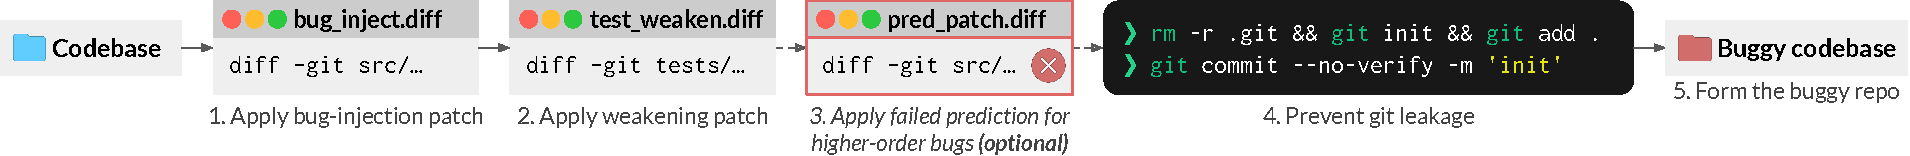
\includegraphics[width=\linewidth]{plots/ssr-bug-construction.pdf}
    \caption{Constructing the buggy codebase from a valid bug artifact.}
    \label{fig:bug-construction}
\end{figure*}

Starting from the original codebase, we first apply \path{bug_inject.diff} to introduce the bug. Next, we apply \path{test_weaken.diff} to hide the bug from the existing test suite.
For higher-order bugs, we additionally apply the failed prediction patch \path{pred_patch.diff} from a prior solver attempt.
Finally, to prevent information leakage through git history, which could otherwise lead to hacking~\cite{swebench_reward_hacking_repo_state_loopholes}, we reinitialize the repository by removing the \path{.git} directory and creating a fresh commit. The resulting buggy codebase forms the solver's starting environment.

\begin{figure*}[t!]
    \centering
    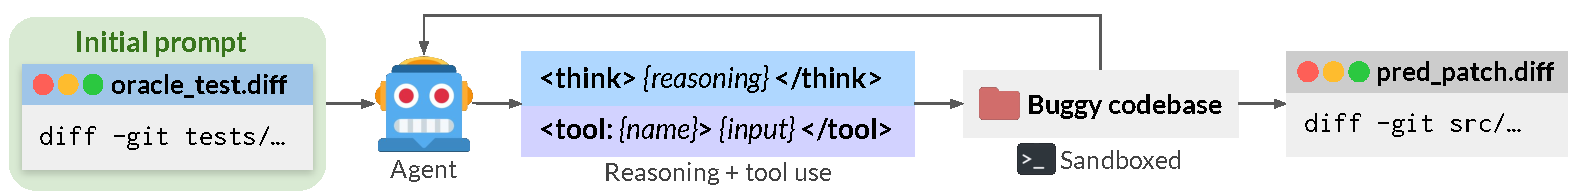
\includegraphics[width=0.85\linewidth]{plots/ssr-solve.pdf}
    \caption{Agentic bug-repair process.}
    \label{fig:bug-repair}
\end{figure*}

\paragraph{Initial prompt.}
In addition to the buggy environment, the agent also needs an initial prompt to understand the task requirements.
We simply provide the agent with a reversed version of the test weakening patch, with an example showed in \cref{fig:weakening}, telling it to satisfy the test requirements while making sure all relevant tests in the codebase can pass without errors.
The detailed prompt template is shown in \cref{sec:apd:prompt_bug_solving}.
Notably, we \textbf{do not synthesize issue descriptions in natural language forms}, as it is difficult to automatically evaluate the quality of free-form natural language text.
Furthermore, high-quality natural language issues are inherently 
scarce compared to the vast synthetic tasks that can be created by bug injection.
As a result, the downstream improvements in issue solving, which operates on natural language issues, purely stem from learning to write test-passing code rather than simple in-domain generalization.

\paragraph{Bug-repair process.}
With the buggy codebase and the initial prompt, the bug-repair process is shown in \cref{fig:bug-repair}.
Starting with the initial prompt, the agent interacts with the sandboxed buggy codebase by performing reasoning and using tools, until it produces a final prediction patch.

For each prediction patch, we evaluate its correctness using the pipeline demonstrated in \cref{fig:pred-patch-eval}.
Beginning with the original codebase, we first tag the current state as \texttt{ssr-original} to preserve a reference 
to the ground-truth repository. We then apply \texttt{bug\_inject.diff} followed by 
\texttt{test\_weaken.diff} to construct the buggy codebase. Next, we apply the predicted patch to the buggy codebase and restore the test files listed in \texttt{test\_files.txt} from the 
\texttt{ssr-original} tag. This restoration step ensures evaluation integrity. Finally, we execute 
\texttt{test\_script.sh} and pipe its output through \texttt{test\_parser.py} 
to obtain a structured mapping of test results in JSON, determining whether the patch successfully resolves the bug.

\begin{figure*}[htb!]
    \centering
    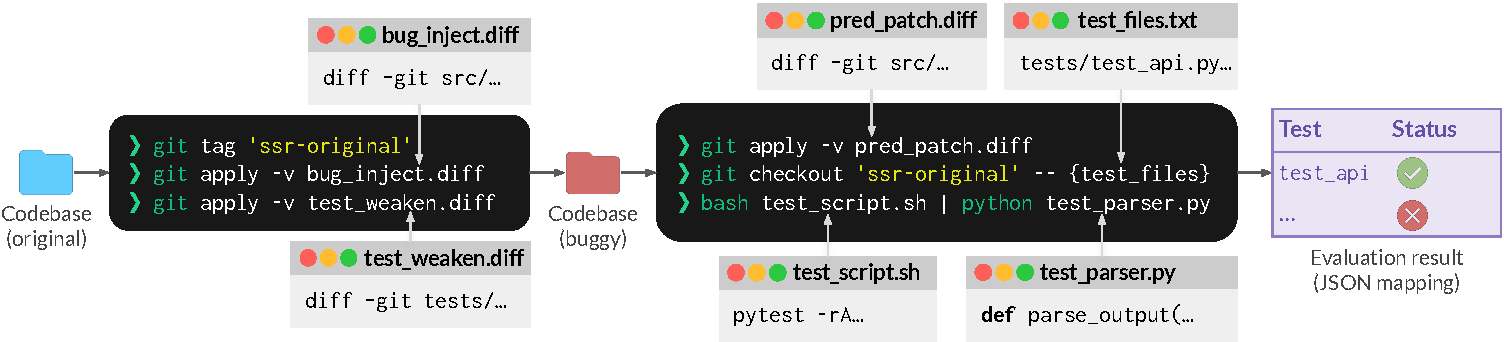
\includegraphics[width=\linewidth]{plots/ssr-eval.pdf}
    \caption{Evaluating the correctness of model-predicted patches.}
    \label{fig:pred-patch-eval}
\end{figure*}

As discussed in \cref{sec:bug_injection}, some solver attempts may fail. These failed attempts are converted into \textbf{higher-order bugs} based on the new bug states derived by the agent.
Higher-order bugs are provided to the solver agent to make additional attempts.
We do not go beyond the second order to prevent a higher likelihood of overlapping with existing bugs.


\paragraph{Reward design.}
For the bug-solving agent, we employ a simple binary reward based on whether all the tests pass after applying the prediction patch:
\begin{equation}
r_{\text{solve}} = \begin{cases}
+1 & \text{if all tests pass,} \\
-1 & \text{otherwise.}
\end{cases}
\end{equation}



